%%
%%

\section*{What is Bacula?}
\label{_ChapterStart41}
\index[general]{Bacula!What is }
\index[general]{What is Bacula? }
\addcontentsline{toc}{section}{What is Bacula?}

{\bf Bacula} is a set of computer programs that permit you (or the system
administrator) to manage backup, recovery, and verification of computer data
across a network of computers of different kinds. In technical terms, it is a
network Client/Server based backup program. Bacula is relatively easy to use
and efficient, while offering many advanced storage management features that
make it easy to find and recover lost or damaged files. Due to its modular
design, Bacula is scalable from small single computer systems to systems
consisting of hundreds of computers located over a large network. 

\subsection*{Who Needs Bacula?}
\index[general]{Who Needs Bacula? }
\index[general]{Bacula!Who Needs }
\addcontentsline{toc}{subsection}{Who Needs Bacula?}

If you are currently using a program such as {\bf tar}, {\bf dump}, or {\bf
bru} to backup your computer data, and you would like a network solution, more
flexibility, or catalog services, Bacula will most likely provide the
additional features you want. However, if you are new to Unix systems or do
not have offsetting experience with a sophisticated backup package, we do not
recommend using Bacula as it is much more difficult to setup and use than {\bf
tar} or {\bf dump}. 

If you are running {\bf Amanda} and would like a backup program that can write
to multiple volumes (i.e. is not limited by your tape drive capacity), Bacula
can most likely fill your needs. In addition, quite a number of our users
report that Bacula is simpler to setup and use than other equivalent programs.


If you are currently using a sophisticated commercial package such as Legato
Networker. ARCserveIT, Arkeia, or PerfectBackup+, you may be interested in
Bacula, which provides many of the same features, and is free software
available under the GNU Version 2 software license. 

\subsection*{Bacula Components or Services}
\index[general]{Bacula Components or Services }
\index[general]{Services!Bacula Components or }
\addcontentsline{toc}{subsection}{Bacula Components or Services}

Bacula is made up of the following five major components or services: 

\addcontentsline{lof}{figure}{Bacula Applications}
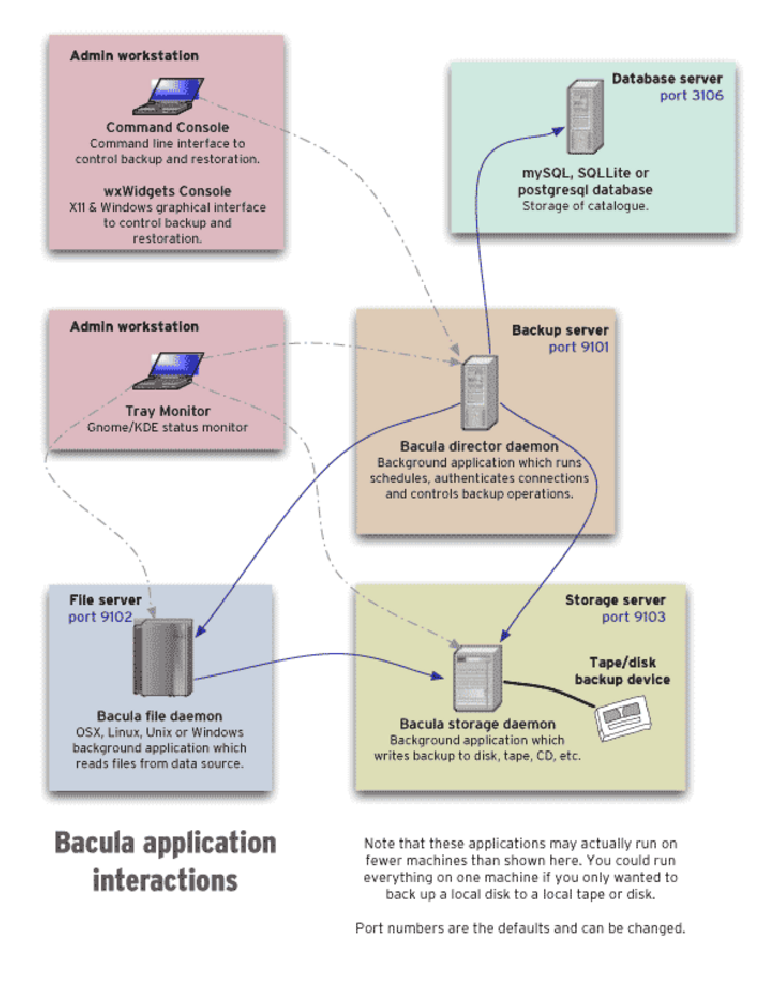
\includegraphics{./bacula-applications.eps} 
(thanks to Aristedes Maniatis for this graphic and the one below) 

\begin{itemize}
\item 
   \label{DirDef}
   {\bf Bacula Director} service consists of the program that  supervises all the
backup, restore, verify and archive operations.  The system administrator uses
the Bacula Director to schedule  backups and to recover files. For more
details see the  Director Services Daemon Design Document in the Bacula
Developer's  Guild.  The Director runs as a daemon or a service (i.e. in the
background). 
\item 
   \label{UADef}
   {\bf Bacula Console} services is the program that allows the  administrator or
user to communicate with the {\bf Bacula Director}  (see above). Currently,
the Bacula Console is available in three  versions. The first and simplest is
to run the Console program in a  shell window (i.e. TTY interface). Most
system administrators will  find this completely adequate. The second version
is a GNOME GUI  interface that for the moment (23 November 2003) is far from
complete,  but quite functional as it has most the capabilities of the shell 
Console. The third version is a wxWidgets GUI with an interactive file 
restore. It also has most the capabilities of the shell console,  allows
command completion with tabulation, and gives you instant  help about the
command you are typing. For more details see the  
\ilink{Bacula Console Design Document}{_ChapterStart23}. 
\item 
   \label{FDDef}
   {\bf Bacula File} services (or Client program) is the software  program that
is installed on the machine to be backed up. It is  specific to the operating
system on which it runs and is responsible  for providing the file attributes
and data when requested by the  Director. The File services are also
responsible for the file  system dependent part of restoring the file
attributes and data  during a recovery operation. For more details see the 
File Services Daemon Design Document in the Bacula Developer's Guide. This 
program runs as a daemon on the machine to be backed up, and in some  of the
documentation, the File daemon is referred to as the Client  (for example in
Bacula's configuration file). In addition to  Unix/Linux File daemons, there
is a Windows File daemon (normally  distributed in binary format). The Windows
File daemon runs on  all currently known Windows versions (95, 98, Me, NT,
2000, XP). 
\item 
   \label{SDDef}
   {\bf Bacula Storage} services consist of the software programs that  perform
the storage and recovery of the file attributes and data to  the physical
backup media or volumes. In other words, the Storage daemon  is responsible
for reading and writing your tapes (or other  storage media, e.g. files). For
more details see the  Storage Services Daemon Design Document in the Bacula
Developer's Guild.  The Storage services runs as a daemon on the machine that
has the  backup device (usually a tape drive). 
\item 
   \label{DBDefinition}
   {\bf Catalog} services are comprised of the software programs  responsible for
maintaining the file indexes and volume databases for  all files backed up.
The Catalog services permit the System  Administrator or user to quickly
locate and restore any desired  file. The Catalog services sets Bacula apart
from simple backup  programs like tar and bru, because the catalog maintains a
record  of all Volumes used, all Jobs run, and all Files saved, permitting 
efficicient restoration and Volume management.  Bacula currently supports
three different databases, MySQL,  PostgreSQL, and SQLite, one of which must
be chosen when building  {\bf Bacula}. There also exists an Internal database,
but it is no  longer supported.  

The three SQL databases currently supported (MySQL, PostgreSQL or SQLite) 
provide quite a number of features,  including rapid indexing, arbitrary
queries, and security. Although  we plan to support other major SQL databases,
the current  Bacula implementation interfaces only to MySQL, PostgreSQL and
SQLite.  For more details see the 
\ilink{Catalog Services Design Document}{_ChapterStart30}.  

The RPMs for MySQL and PostgreSQL ship as part of the Linux RedHat release, 
or building it from the source is quite easy, see the  
\ilink{ Installing and Configuring MySQL}{_ChapterStart} chapter  of
this document for the details. For more information on MySQL,  please see: 
\elink{www.mysql.com}{http://www.mysql.com}.  Or see the 
\ilink{ Installing and Configuring PostgreSQL}{_ChapterStart10}
chapter of this document for the details. For more  information on PostgreSQL,
please see: 
\elink{www.postgresql.org}{http://www.postgresql.org}.  

Configuring and building SQLite is even easier. For the details  of
configuring SQLite, please see the 
\ilink{ Installing and Configuring SQLite}{_ChapterStart33} chapter
of this document. 
\item 
   \label{MonDef}
   {\bf Bacula Monitor} services is the program that allows the  administrator or
user to watch current status of {\bf Bacula Directors},  {\bf Bacula File
Daemons} and {\bf Bacula Storage Daemons}  (see above). Currently, only a GTK+
version is available, which  works with Gnome and KDE (or any window manager
that supports the  FreeDesktop.org system tray standard). 
\end{itemize}

To perform a successful save or restore, the following four daemons must be
configured and running: the Director daemon, the File daemon, the Storage
daemon, and MySQL, PostgreSQL or SQLite. 

\subsection*{Bacula Configuration}
\index[general]{Configuration!Bacula }
\index[general]{Bacula Configuration }
\addcontentsline{toc}{subsection}{Bacula Configuration}

In order for Bacula to understand your system, what clients you want backed
up, and how, you must create a number of configuration files containing
resources (or objects). The following presents an overall picture of this: 

\addcontentsline{lof}{figure}{Bacula Objects}
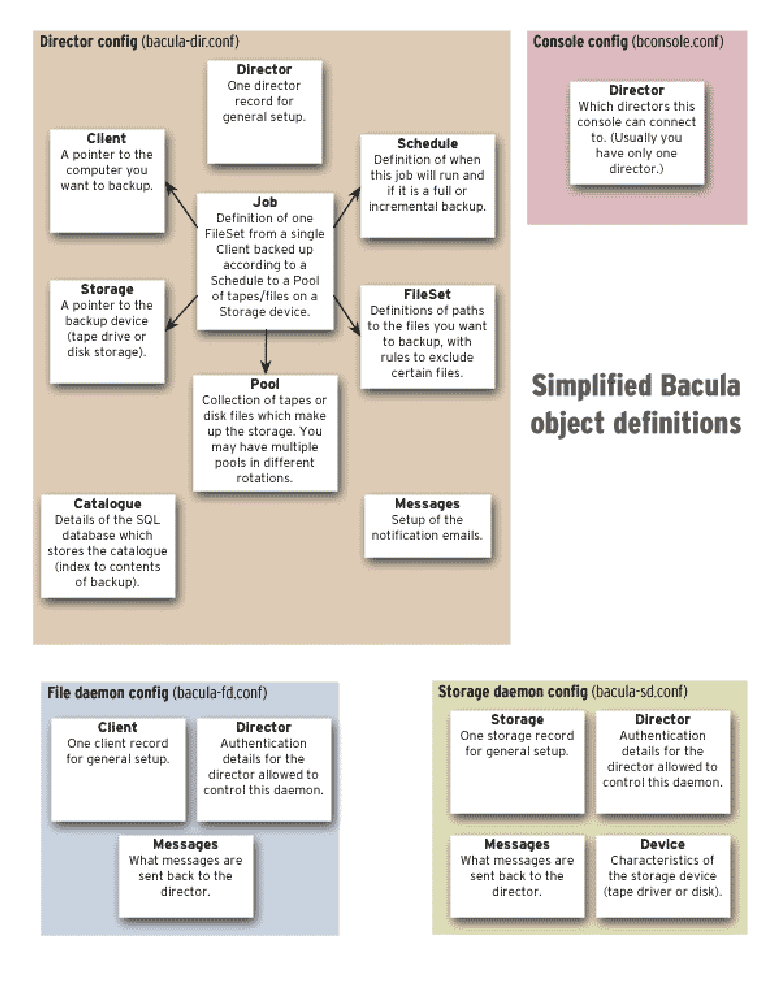
\includegraphics{./bacula-objects.eps} 

\subsection*{Conventions Used in this Document}
\index[general]{Conventions Used in this Document }
\index[general]{Document!Conventions Used in this }
\addcontentsline{toc}{subsection}{Conventions Used in this Document}

{\bf Bacula} is in a state of evolution, and as a consequence, this manual
will not always agree with the code. If an item in this manual is preceded by
an asterisk (*), it indicates that the particular feature is not implemented.
If it is preceded by a plus sign (+), it indicates that the feature may be
partially implemented. 

If you are reading this manual as supplied in a released version of the
software, the above paragraph holds true. If you are reading the online
version of the manual, 
\elink{ www.bacula.org/manual}{http://www.bacula.org/manual}, please bear in
mind that this version describes the current version in development (in the
CVS) that may contain features not in the released version. Just the same, it
generally lags behind the code a bit. 

\subsection*{Quick Start}
\index[general]{Quick Start }
\index[general]{Start!Quick }
\addcontentsline{toc}{subsection}{Quick Start}

To get Bacula up and running quickly, we recommend that you first scan the
Terminology section below, then quickly review the next chapter entitled 
\ilink{The Current State of Bacula}{_ChapterStart2}, then the 
\ilink{Getting Started with Bacula}{_ChapterStart37}, which will
give you a quick overview of getting Bacula running. After which, you should
proceed to the chapter on 
\ilink{Installing Bacula}{_ChapterStart17}, then 
\ilink{How to Configure Bacula}{_ChapterStart16}, and finally the
chapter on 
\ilink{ Running Bacula}{_ChapterStart1}. 

\subsection*{Terminology}
\index[general]{Terminology }
\addcontentsline{toc}{subsection}{Terminology}

To facilitate communication about this project, we provide here the
definitions of the terminology that we use. 

\begin{description}

\item [Administrator]
   \index[fd]{Administrator }
   The person or persons responsible for administrating  the Bacula system. 

\item [Backup]
   \index[fd]{Backup }
   We use the term {\bf Backup} to refer to a  Bacula Job that saves files. 

\item [Bootstrap File]
   \index[fd]{Bootstrap File }
   The bootstrap file is an ASCII file  containing a compact form of commands
that allow Bacula or  the stand-alone file extraction utility ({\bf bextract})
to  restore the contents of one or more Volumes, for example, the  current
state of a system just backed up. With a bootstrap file,  Bacula can restore
your system without a Catalog. You can  create a bootstrap file from a Catalog
to extract any file or  files you wish. 

\item [Catalog]
   \index[fd]{Catalog }
   The Catalog is used to store summary information  about the Jobs, Clients, and
Files that were backed up and on  what Volume or Volumes. The information
saved in the Catalog  permits the administrator or user to determine what jobs
were  run, their status as well as the important characteristics  of each file
that was backed up. The Catalog is an online resource,  but does not contain
the data for the files backed up. Most of  the information stored in the
catalog is also stored on the  backup volumes (i.e. tapes). Of course, the
tapes will also have  a copy of the file in addition to the File Attributes
(see below).  

The catalog feature is one part of Bacula that distinguishes  it from simple
backup and archive programs such as {\bf dump}  and {\bf tar}.  

\item [Client]
   \index[fd]{Client }
   In Bacula's terminology, the word Client  refers to the machine being backed
up, and it is synonymous  with the File services or File daemon, and quite
often, we  refer to it as the FD. A Client is defined in a configuration  file
resource. 

\item [Console]
   \index[fd]{Console }
   The program that interfaces to the Director allowing  the user or system
administrator to control Bacula. 

\item [Daemon]
   \index[fd]{Daemon }
   Unix terminology for a program that is always present in  the background to
carry out a designated task. On Windows systems, as  well as some Linux
systems, daemons are called {\bf Services}. 

\item [Directive]
   \index[fd]{Directive }
   The term directive is used to refer to a statement  or a record within a
Resource in a configuration file that  defines one specific thing. For
example, the {\bf Name} directive  defines the name of the Resource. 

\item [Director]
   \index[fd]{Director }
   The main Bacula server daemon that schedules and directs all  Bacula
operations. Occassionally, we refer to the Director as DIR. 

\item [Differential]
   \index[fd]{Differential }
   A backup that includes all files changed since the last  Full save started.
Note, other backup programs may define this differently. 

\item [File Attributes]
   \index[fd]{File Attributes }
   The File Attributes are all the information  necessary about a file to
identify it and all its properties such as  size, creation date, modification
date, permissions, etc. Normally, the  attributes are handled entirely by
Bacula so that the user never  needs to be concerned about them. The
attributes do not include the  file's data. 

\item [File Daemon]
   \index[fd]{File Daemon }
   The daemon running on the client  computer to be backed up. This is also
referred to as the File  services, and sometimes as the Client services or the
FD. 

\item [
   \label{FileSetDef}
   FileSet]
\index[fd]{a name }
A FileSet is a Resource contained in a configuration  file that defines the
files to be backed up. It consists  of a list of included files or
directories, a list of excluded files, and  how the file is to be stored
(compression, encryption, signatures).  For more details, see the 
\ilink{FileSet Resource definition}{FileSetResource}  in the
Director chapter of this document. 

\item [Incremental]
   \index[fd]{Incremental }
   A backup that includes all files changed since the  last Full, Differential,
or Incremental backup started. It is normally  specified on the {\bf Level}
directive within the Job resource  definition, or in a Schedule resourc. 

\item [
   \label{JobDef}
   Job]
\index[fd]{a name }
A Bacula Job is a configuration resource that defines  the work that Bacula
must perform to backup or restore a particular  Client. It consists of the
{\bf Type} (backup, restore, verify,  etc), the {\bf Level} (full,
incremental,...), the {\bf FileSet},  and {\bf Storage} the files are to be
backed up (Storage device,  Media Pool). For more details, see the 
\ilink{Job Resource definition}{JobResource} in the  Director
chapter of this document. 

\item [Monitor]
   \index[fd]{Monitor }
   The program that interfaces to the all the daemons  allowing the user or
system administrator to monitor Bacula status. 

\item [Resource]
   \index[fd]{Resource }
   A resource is a part of a configuration file that  defines a specific unit of
information that is available to Bacula.  For example, the {\bf Job} resource
defines all the properties of  a specific Job: name, schedule, Volume pool,
backup type, backup  level, ... 

\item [Restore]
   \index[fd]{Restore }
   A restore is a configuration resource that  describes the operation of
recovering a file (lost or damaged) from  backup media. It is the inverse of a
save, except that in most  cases, a restore will normally have a small set of
files to restore,  while normally a Save backs up all the files on the system.
Of  course, after a disk crash, Bacula can be called upon to do  a full
Restore of all files that were on the system. 

\item [Schedule]
   \index[fd]{Schedule }
   A Schedule is a configuration resource that  defines when the Bacula Job will
be scheduled for  execution. To use the Schedule, the Job resource will refer
to  the name of the Schedule. For more details, see the 
\ilink{Schedule Resource definition}{ScheduleResource} in the
Director chapter of this document. 

\item [Service]
   \index[fd]{Service }
   This is Windows terminology for a {\bf daemon} -- see  above. It is now
frequently used in Unix environments as well. 

\item [Storage Coordinates]
   \index[fd]{Storage Coordinates }
   The information returned from the  Storage Services that uniquely locates a
file on a backup medium. It  consists of two parts: one part pertains to each
file saved, and the  other part pertains to the whole Job. Normally, this
information is  saved in the Catalog so that the user doesn't need specific
knowledge  of the Storage Coordinates. The Storage Coordinates include the 
File Attributes (see above) plus the unique location of the information on 
the backup Volume. 

\item [Storage Daemon]
   \index[fd]{Storage Daemon }
   The Storage daemon, sometimes referred to as  the SD, is the code that writes
the attributes and data to a storage  Volume (usually a tape or disk). 

\item [Session]
   \index[sd]{Session }
   Normally refers to the internal conversation between  the File daemon and the
Storage daemon. The File daemon opens a  {\bf session} with the Storage daemon
to save a FileSet, or to restore  it. A session has a one to one
correspondence to a Bacula Job (see  above). 

\item [Verify]
   \index[sd]{Verify }
   A verify is a job that compares the current file  attributes to the attributes
that have previously been stored in the  Bacula Catalog. This feature can be
used for detecting changes to  critical system files similar to what {\bf
Tripwire} does. One  of the major advantages of using Bacula to do this is
that  on the machine you want protected such as a server, you can run  just
the File daemon, and the Director, Storage daemon, and Catalog  reside on a
different machine. As a consequence, if your server is  ever compromised, it
is unlikely that your verification database  will be tampered with.  

Verify can also be used to check that the most recent Job  data written to a
Volume agrees with what is stored in the Catalog  (i.e. it compares the file
attributes), *or it can check the  Volume contents against the original files
on disk. 

\item [*Archive]
   \index[fd]{*Archive }
   An Archive operation is done after a Save, and it  consists of removing the
Volumes on which data is saved from active  use. These Volumes are marked as
Archived, and many no longer be  used to save files. All the files contained
on an Archived Volume  are removed from the Catalog. NOT YET IMPLEMENTED. 

\item [*Update]
   \index[fd]{*Update }
   An Update operation causes the files on the remote  system to be updated to be
the same as the host system. This is  equivalent to an {\bf rdist} capability.
NOT YET IMPLEMENTED.  

\item [Retention Period]
   \index[fd]{Retention Period }
   There are various kinds of retention  periods that Bacula recognizes. The most
important are the  {\bf File} Retention Period, {\bf Job} Retention Period,
and the  {\bf Volume} Retention Period. Each of these retention periods 
applies to the time that specific records will be kept in the  Catalog
database. This should not be confused with the time that  the data saved to a
Volume is valid. 

The File Retention Period  determines the time that File records are kept in
the catalog  database. This period is important because the volume of the 
database File records by far use the most storage space in the  database. As a
consequence, you must ensure that regular  ``pruning'' of the database file
records is done. (See  the Console {\bf retention} command for more details on
this  subject). 

The Job Retention Period is the length of time that  Job records will be kept
in the database. Note, all the File  records are tied to the Job that saved
those files. The File  records can be purged leaving the Job records. In this
case,  information will be available about the jobs that ran, but not the 
details of the files that were backed up. Normally, when a Job  record is
purged, all its File records will also be purged. 

The  Volume Retention Period is the minimum of time that a Volume will be 
kept before it is reused. Bacula will normally never  overwrite a Volume that
contains the only backup copy of a file.  Under ideal conditions, the Catalog
would retain entries for all  files backed up for all current Volumes. Once a
Volume is  overwritten, the files that were backed up on that Volume are 
automatically removed from the Catalog. However, if there is a very  large
pool of Volumes or a Volume is never overwritten, the Catalog  database may
become enormous. To keep the Catalog to a manageable  size, the backup
information should removed from the Catalog after  the defined File Retention
Period. Bacula provides the  mechanisms for the catalog to be automatically
pruned according to  the retention periods defined. 

\item [Scan]
   \index[sd]{Scan }
   A Scan operation causes the contents of a Volume or a  series of Volumes to be
scanned. These Volumes with the information  on which files they contain are
restored to the Bacula Catalog.  Once the information is restored to the
Catalog, the files contained  on those Volumes may be easily restored. This
function is  particularly useful if certain Volumes or Jobs have exceeded 
their retention period and have been pruned or purged from the  Catalog.
Scanning data from Volumes into the Catalog is done  by using the {\bf bscan}
program. See the 
\ilink{ bscan section}{bscan} of the Bacula Utilities Chapter of
this manual  for more details. 

\item [Volume]
   \index[sd]{Volume }
   A Volume is an archive unit, normally a tape or  a named disk file where
Bacula stores the data from one or more  backup jobs. All Bacula Volumes have
a software label written to  the Volume by Bacula so that it identify what
Volume it is really  reading. (Normally there should be no confusion with disk
files,  but with tapes, it is easy to mount the wrong one). 
\end{description}

\subsection*{What Bacula is Not}
\index[general]{Not!What Bacula is }
\index[general]{What Bacula is Not }
\addcontentsline{toc}{subsection}{What Bacula is Not}

{\bf Bacula} is a backup, restore and verification program and is not a
complete disaster recovery system in itself, but it can be a key part of one
if you plan carefully and follow the instructions included in the 
\ilink{ Disaster Recovery}{_ChapterStart38} Chapter of this manual. 

With proper planning, as mentioned in the Disaster Recovery chapter {\bf
Bacula} can be a central component of your disaster recovery system. For
example, if you have created an emergency boot disk, a Bacula Rescue disk to
save the current partitioning information of your hard disk, and maintain a
complete Bacula backup, it is possible to completely recover your system from
``bare metal''. 

If you have used the {\bf WriteBootstrap} record in your job or some other
means to save a valid bootstrap file, you will be able to use it to extract
the necessary files (without using the catalog or manually searching for the
files to restore). 

\subsection*{Interactions Between the Bacula Services}
\index[general]{Interactions Between the Bacula Services }
\index[general]{Services!Interactions Between the Bacula }
\addcontentsline{toc}{subsection}{Interactions Between the Bacula Services}

The following block diagram shows the typical interactions between the Bacula
Services for a backup job. Each block represents in general a separate process
(normally a daemon). In general, the Director oversees the flow of
information. It also maintains the Catalog. 

\addcontentsline{lof}{figure}{Interactions between Bacula Services}
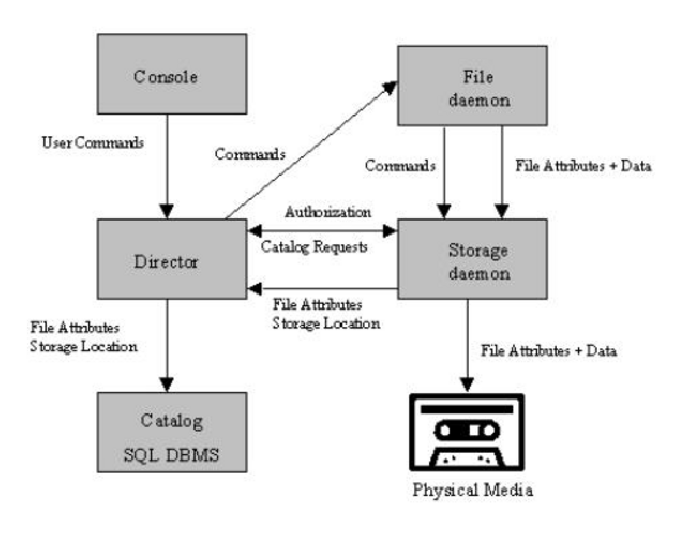
\includegraphics{./flow.eps} 
